% vim: set tw=78 sts=2 sw=2 ts=8 aw et ai:

\subsection{Corpus, Smoothing and Historical Relevance}

The full Google Books Ngram Corpus has been made freely available by Google. In this paper, only statistics for 1-grams are used. More specifically, the analysis shall be based on the time series it provides for each word, mapping the year of publishing to the frequency of the n-gram in books written in that year. In order to deny the negative effect that the natural increase in books published each year may have on the relevance of the time series, the model's input shall instead be the time series of normalized frequencies. The time spanned by the series is between $1500$ and $2008$.

Although much effort has been put into ensuring the quality of the Google Books Ngram Corpus, it still contains noise from sources such as erroneous date of publication. In order to mitigate this effect, the simple solution is to smooth the series. More formally, say that the time series for a given word $w_i$ is denoted by $\left\{ s_{i, t} \right\}_{t = 1500}^{2008}$. Then, the smoothed series with window $k$ is given by

\begin{align}
\label{eq:smooth-series}
u_{k} \left( i, t \right) = \frac{\sum_{d = -k}^{k} s_{i, t + d}}{2k + 1}, \, \forall t \in \overline{1500 + d, 2008 - d}.
\end{align}

From now on, all references to $\left\{ s_{i, t} \right\}$ shall instead refer to the associated smoothed series $u_k$ defined in equation \eqref{eq:smooth-series} above, for a value of $k$ that will be later empirically determined.

The data provided by the Google Books Ngram Corpus is immense (only the 1-grams have a size of about 30 GB), so trying to identify historic events using all of the raw data seems to be an intractable problem. In order to solve this issue, I have opted to perform a preliminary transformation on the data, with the purpose of reducing the size to a more manageable order of magnitude. Of course, the transformation should retain the property of historical relevance of an n-gram in a given year, so the subsequent analysis can correctly model the influence of historic events on texts. Regarding the structure of the time series, it should transform a time series of normalized frequencies (real numbers between $0$ and $1$) to a time series reflecting historical relevance on a discrete scale, for example the integers in $\left[ 0, 10 \right]$, where $0$ would reflect lack of historical relevance of the n-gram in that year and $10$ would reflect an n-gram that basically defines that year. Due to the implicit localized nature of historic events, any given n-gram should attain historical relevance only within a small time frame. Thus, most of the entries in the reduced time series should be zero, leading to a highly sparse representation. Therefore, not only is this transformation useful from a practical point of view (it drastically reduces the computational resources required for the analysis), but it also has theoretical arguments that it maps well to the task of historic events identification.

The exact scale used for the reduced time series is not fixed beforehand and it is worth discussing its influence. Thus, representing historical relevance on a binary scale leads to an extremely sparse model that can be analyzed very fast, but that will lead to mediocre results. Increasing the number of degrees of relevance will lead to better and better representations and consequently to results of higher quality. There is an unavoidable trade-off to be made here, namely the one between the time necessary to run model and its quality, so the scale will be practically limited by the amount of computational resources available for the subsequent analysis of the reduced time series.

\subsection{Historical Relevance Algorithms}
\label{sec:historical-relevance-algorithms}
% vim: set tw=78 sts=2 sw=2 ts=8 aw et ai:

In order to explain the algorithms used for determining historical relevance, I shall first analyze a typical time series, using as example a word that carries a heavy influence on history: war.

\begin{figure}
\centering
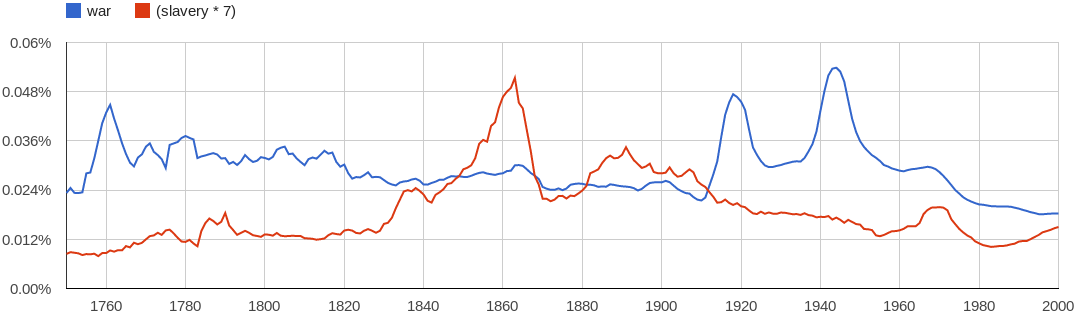
\includegraphics[max size={\textwidth}{\textheight}]{war-series}
\caption{Ngram time series for war}
\label{fig:war-series}
\end{figure}

Taking a look at \autoref{fig:war-series}, the first feature of the plot that can be noticed is the presence of several well-defined peaks. One can immediately make the connection of the three obvious peaks with historic events: the first one, between $1755$ and $1765$, corresponds to the Seven Years' War, which involved most of Europe, North America, Central America, West Africa and India; the second one, between $1910$ and $1926$, is clearly caused by World War I, which was centred in Europe and involved around 70 million military personnel; the third one, between $1936$ and $1953$, is determined by World War II, which was fought by most of the planet's nations and resulted into upwards of 50 million casualties.

However, a closer inspection reveals the presence of further peak-like shapes, some of which can be identified with major wars in history. Between $1775$ and $1783$ took place the American Revolutionary War, which not only involved Great Britain and the United States, but also France, Netherlands and Spain. Between $1860$ and $1871$ one can note another peak most probably corresponding to the American Civil War, which had the abolition of slavery as one of its goals. More recently, between $1961$ and $1978$, there is a shape vaguely resembling a peak most likely generated by the Vietnam War, fought between North Vietnam and its communist allies on the one side and South Vietnam and the United States on the other. From these observations, it is clear that the analysis of only one n-gram, war, cannot be solely used to determine the major wars that have taken place in our history. The shape of a singular plot can only reveal so much information, but by determining historical relevance for different n-grams and correlating the results, one can viably get a picture of a historic event.

\begin{figure}
\centering
\includegraphics[max size={\textwidth}{\textheight}]{comparative-series}
\caption{Ngram time series for atomic, trench and slavery}
\label{fig:comparative-series}
\end{figure}

As a prime example of the above idea, \autoref{fig:comparative-series} presents a comparative analysis of the following 3 n-grams: atomic, trench and slavery. Note that I have taken the freedom to scale the three plots for easier visualization, as in the end it is only the shape of the graph that is under scrutiny. One can notice three surges in the frequency time series. Firstly, slavery has a very sharp triangular peak between $1842$ and $1871$, which includes the American Civil War, known for the fact it had slavery as a core issue. Secondly, trench has a significant peak between $1911$ and $1925$, corresponding to World War I, known for the heavy use of trench warfare. Lastly, atomic also has a wide peak between $1939$ and $1972$, motivated by the development of the atomic bomb, its use in World War II and its potential use in the Cold War.

For this analysis to be tractable on the large amounts of data available in the corpus, one must come up with an algorithm for peak detection. It has to be not only reliable, but also has to run fast enough so it can cope with the limited amount of resources. The trade-off that can be made in this situation is between complexity of the peak detection algorithm and the amount of data that can be actually processed. At one extreme, if the algorithm is too simple, it can process all the data, but the results will probably be of inferior quality. At the other, if the algorithm is too complicated, it can only process a negligible portion of the corpus, so again the results are likely to be mediocre. Another decision to be made here is selecting the corpus subset that is left out. The intuitive solution is to leave out the least frequent n-grams, the heuristic being that rare words are pretty unlikely to be connected with a major historic event.

A further requirement for the algorithm is the capability of meaningfully characterizing a peak. Thus, besides determining the period of time that a peak occurred, it also needs to quantitatively measure the historical relevance of that peak. In the example of the n-gram war, the three large peaks should be assigned a high historical relevance. In regard to the other three lesser peaks, it is debatable whether the algorithm should even detect them, but in case it does, they should be assigned a low historical relevance. Furthermore, the value of the historical relevance needs not be constant over the entire peak. Instead, advanced schemes can use a variable historical relevance, perhaps assigning more to the center of the peak and less to the outskirts of the peak.

\subsubsection{Double Change Peak Detection}

Arguably the simplest way of detecting peaks is by making use of the fact that peaks usually consist of a period of abrupt increase, followed by another period of abrupt decrease. A computationally inexpensive method for doing this is detecting periods of time marked by a double change of the time series in the same direction, either increasing or decreasing.

Formally, we say that a time series $\left\{ s_{i, t} \right\}$ suffers a double increase of magnitude $x \in \left[ 0, 1 \right)$ at time $t$ if:

\begin{align}
\label{eq:double-increase}
s_{i, t} > \left( 1 + x \right) s_{i, t - 1} \textrm{ and } s_{i, t + 1} > \left( 1 + x \right) s_{i, t}.
\end{align}

Similarly, we say that a time series $\left\{ s_{i, t} \right\}$ suffers a double decrease of magnitude $x \in \left[ 0, 1 \right)$ at time $t$ if:

\begin{align}
\label{eq:double-decrease}
s_{i, t} < \left( 1 - x \right) s_{i, t - 1} \textrm{ and } s_{i, t + 1} < \left( 1 - x \right) s_{i, t}.
\end{align}

One problem that may appear with these definitions is that, for example, during the ascent part of the peak, at often times the increase rate will randomly dip below a certain threshold, causing the algorithm to miss a valuable information. To this end, I have also introduced the notion of single increase of magnitude $x \in \left[ 0, 1 \right)$:

\begin{align}
\label{eq:single-increase}
s_{i, t} &> \left( 1 + 2x \right) s_{i, t - 1}.
\end{align}

Similarly, the notion of single decrease of magnitude $x \in \left[ 0, 1 \right)$ is defined as follows:

\begin{align}
\label{eq:single-decrease}
s_{i, t} &< \left( 1 - 2x \right) s_{i, t - 1}.
\end{align}

As can be noticed, the latter two notions use a factor of $2x$ in the formulas instead of the $x$ used in the double change formulas. The reasoning behind this is that although we don't want to miss any potential peaks, single changes in the time series can sometimes not be part of a peak. Therefore, I made it harder for single changes to achieve a certain magnitude, while still making sure that the original problem was also solved.

The magnitude $m_{i, t}$ of the change around a point $t$ in a time series $\left\{ s_{i, t} \right\}$ is defined as the maximum between the magnitude of the double change and the magnitude of the single change at that point. From this, the historical relevance is computed as follows:

\begin{align}
\label{eq:double-change-relevance}
r_{i, t} &= \min \left( \left\lfloor 10 m_{i, t} \right\rfloor, 9 \right).
\end{align}

The relevance value is thus an integer proportional to the magnitude $m_{i, t}$. However, an artificial cap has been placed on this value, because n-grams can grow very fast, especially when a new term is born. This has the positive effect of not overemphasizing the exploding word.

\subsubsection{Linear Model Peak Detection}

Drawing on the previous idea of periods of abrupt increase and decrease, one can also use a linear model for approximating portions of the time series. The core of this approach is to fit lines to the graph of the time series using linear regression, by considering larger and larger intervals until the error rises above a given threshold.

\begin{algorithm}

\begin{algorithmic}[1]
\For { $i \in 1 \to \left| \textrm{Words} \right|$ }
    \For { $t \in 1500 \to 2008$ }
        \State $s_{i, t} = \frac{s_{i, t} - \mu_i}{\sigma_i}$
    \EndFor
\EndFor
\For { $i \in 1 \to \left| \textrm{Words} \right|$ }
    \State $u \gets 1500$
    \For { $t \in 1501 \to 2008$ }
        \State $a, b, err \gets \textrm{lm} \left( \left\{ s{i, k}_{k = u}^t \right\} \right)$
        \Comment { Parameters and error of the model $y = ax + b$ }
        \If { $\log(err) >= -5$ }
            \State $m_i \left( u, t \right) \gets 2 \cdot \left( 3 + \log \left| a \right| \right)$
            \State $u \gets t$
        \EndIf
    \EndFor
\EndFor
\end{algorithmic}

\caption{Linear Model Peak Detection Algorithm}
\label{alg:linear-model}

\end{algorithm}

As can be noticed in Algorithm \autoref{alg:linear-model}, the series is first transformed using the standard score, such that, after the transformation, its mean shall be 0 and its variance 1. This is a standard step used for preparing the data for linear regression. Upon finding a maximal interval fitted by a line within a small error, the magnitude of the change on that interval is defined as a linear function of the logarithm of the slope (actually, the absolute value of that slope, since it can also be negative). This choice reflects a wide range of values that the slope can take, forming a sort of heavy-tailed distribution. Taking the logarithm of the slope cancels the effect of the heavy tail and allows for interesting statistics to be collected.

Since taking logarithms eliminates the possibility of ridiculously high magnitudes, the historical relevance for $w_i$ can simply be computed as follows:

\begin{align}
\label{eq:linear-model-relevance}
r_{i, t} &= \max \left( \left\lfloor m_{i, t} \right\rfloor, 0 \right).
\end{align}

\subsubsection{Gaussian Model Peak Detection}

Another completely different idea for peak detection is to notice that peaks are usually shaped like a Gaussian distribution, i.e. they are bell-shaped. So, let's consider a time interval $\left[ l, r \right] \subseteq \left[ 1500, 2008 \right]$ and the time series for some word $w_i$ on that interval, $\left\{ s_{i, t} \right\}_{t=l}^{r}$. Since we want to approximate the series by a normal distribution, it should be probably normalized to that it sums to 1. However, this is not enough, since a Gaussian has an infimum of 0, while a peak can be offset by a significant value. This offset is of course computed as the minimum value of the time series on the given interval. Thus, we define the normalized time series $\left\{ g_{i, t} \right\}_{t=l}^{r}$ as:

\begin{align}
\label{eq:gaussian-normalization}
g_{i, t} &= \frac{s_{i, t} - \min_{p \in \overline{l, r}} s_{i, p}}{\sum_{q = l}^{r} \left( s_{i, q} - \min_{p \in \overline{l, r}} s_{i, p} \right)}.
\end{align}

This is approximated by a normal distribution $N \left( \mu, \sigma \right)$ with the following parameters:

\begin{align}
\label{eq:mu-gaussian-model}
\mu &= \frac{\sum_{t=l}^{r} g_{i, t} t}{r - l + 1}, \\
\label{eq:sigma-gaussian-model}
\sigma^2 &= \frac{\sum_{t=l}^{r} g_{i, t} \left( t - \mu \right)^2}{r - l + 1}.
\end{align}

In order to compute the similarity between $g_{i, t}$ and $N \left( \mu, \sigma \right)$, a variation on the earth mover's distance \cite{rubner98metric} shall be used. Although the former probability distribution is discrete, while the latter is continuous, we shall nonetheless assume that the latter is also discrete by considering only its values in the points $t \in \overline{l, r}$.

\begin{algorithm}

\begin{algorithmic}[1]
\Require $l \geq 1500, r \leq 2008$
\State $acc \gets 0$
\State $distance \gets 0$
\For { $t \in l \to r$ }
    \State $acc \gets acc + g_{i, t} - \frac{1}{\sqrt{2 \pi} \cdot \sigma} \cdot \exp \left( - \frac{\left( t - \mu \right)^2}{2 \sigma^2} \right)$
    \State $distance \gets distance + \left| acc \right|$
\EndFor
\State \Return $distance$
\end{algorithmic}

\caption{Earth Mover's Distance Algorithm}
\label{alg:emd}

\end{algorithm}

The well-known Algorithm \autoref{alg:emd} is based on the idea of treating the value of a probability distribution at a certain point as the amount of dirt found at that distance. Then the distance between two distributions is equal to the minimum amount of work required for transforming a distribution into the other, where work is defined as the amount of dirt moved times the distance it is moved. In general, this is equivalent to the assignment problem, so it can be solved using the Hungarian algorithm. However, in the one-dimensional case, the greedy algorithm presented above works.

In the case of modeling peaks with Gaussian distributions, unfortunately we have to consider all possible intervals $\left[ l, r \right] \subseteq \left[ 1500, 2008 \right]$, which leads to quadratic complexity in the number of invocations of the earth mover's distance algorithm, which is itself linear in the length of the interval. Overall, this leads to a total $O \left( \max(r) - \min(l) \right)^3$ complexity. In order to bring this down an order of magnitude, one needs a heuristic to decide if a probability distribution even remotely looks like a Gaussian bell. To this end, I have chosen to use kurtosis:

\begin{align}
\label{eq:kurtosis}
\gamma_2 &= \frac{\mu_4}{\sigma^4} - 3.
\end{align}

Here, $\mu_4$ is the fourth moment about the mean:

\begin{align}
\label{eq:4th-moment}
\mu_4 &= \frac{\sum_{t=l}^{r} \left( g_{i, t} - \mu \right)^4}{r - l + 1}.
\end{align}

As evidenced in \cite{balanda88kurtosis}, in the case of symmetric distributions, kurtosis can be viewed as an approximate measure of peakedness, with the normal distribution having a kurtosis of 0. Furthermore, kurtosis can be computed, with trivial preprocessing of partial sums, in constant time for any interval $\left[ l, r \right]$. Thus, by imposing a tight limit on the absolute value of the kurtosis, such as $0.05$, the complexity of processing a time series drops heavily and thus one can process even more of them in total.

After that, from the remaining intervals we select the ones that have an earth mover's distance to their corresponding Gaussian distributions lower than $0.3$. A potential problem that can appear is that the intervals may intersect. This can be avoided by first sorting the intervals in increasing order of the earth mover's distance and then processing them one by one. Intervals that intersect previously processed ones are simply ignored, which both ensures that the intervals are disjoint and that only the highest quality peaks are chosen.

Now we compute the magnitude of the change corresponding to an interval $\left[ l, r \right]$ as the percentage with which the Gaussian peak increases from its smallest value to its largest value. The minimum value is computed as a statistic from the original series, while the largest value is derived from the largest value of the Gaussian distribution (which occurs exactly at its mean):

\begin{align}
\label{eq:gaussian-magnitude}
m_i \left( l, r \right) &= \frac{N \left( \mu, \sigma \right) \left( \mu \right) \cdot \sum_{q = l}^{r} \left( s_{i, q} - \min_{p \in \overline{l, r}} s_{i, p} \right)}{\min_{p \in \overline{l, r}} s_{i, p}}.
\end{align}

One way to define historical relevance in this case is to assign it a constant value on the interval, proportional to the magnitude:

\begin{align}
\label{eq:gaussian-model-constant-relevance}
r_{i, t} &= \left\lfloor 10 \cdot \min \left( m_i \left( l, r \right), 1) \right) \right\rfloor, \, \forall t \in \left[ l, r \right].
\end{align}

An alternative way is to assign variable relevance, such that it also forms a Gaussian bell. The formula, that also includes a widening parameter $w \in \left[ 1, \infty \right)$, is as follows:

\begin{align}
\label{eq:gaussian-model-variable-relevance}
r_{i, t} \left( w \right) &= \left\lfloor 10 \cdot \min \left( m_i \left( l, r \right), 1) \right) \right\rfloor \cdot \frac{N \left( \mu, w \sigma \right) \left( t \right)}{N \left( \mu, w \sigma \right) \left( \mu \right)}, \, \forall t \in \left[ l, r \right].
\end{align}

One can note that when $w \to \infty$, \autoref{eq:gaussian-model-variable-relevance} actually converges to \autoref{eq:gaussian-model-constant-relevance}. The idea behind the parameter $w$ is that both extremes are likely to give poor performance: for $w = 1$, too little relevance is assigned to the tails of the distribution, while for $w \to \infty$ too much relevance is assigned to the tails of the distribution. By considering intermediate values one is likely to obtain higher quality results.

\subsubsection{Graphical Analysis}

\begin{figure}
\centering
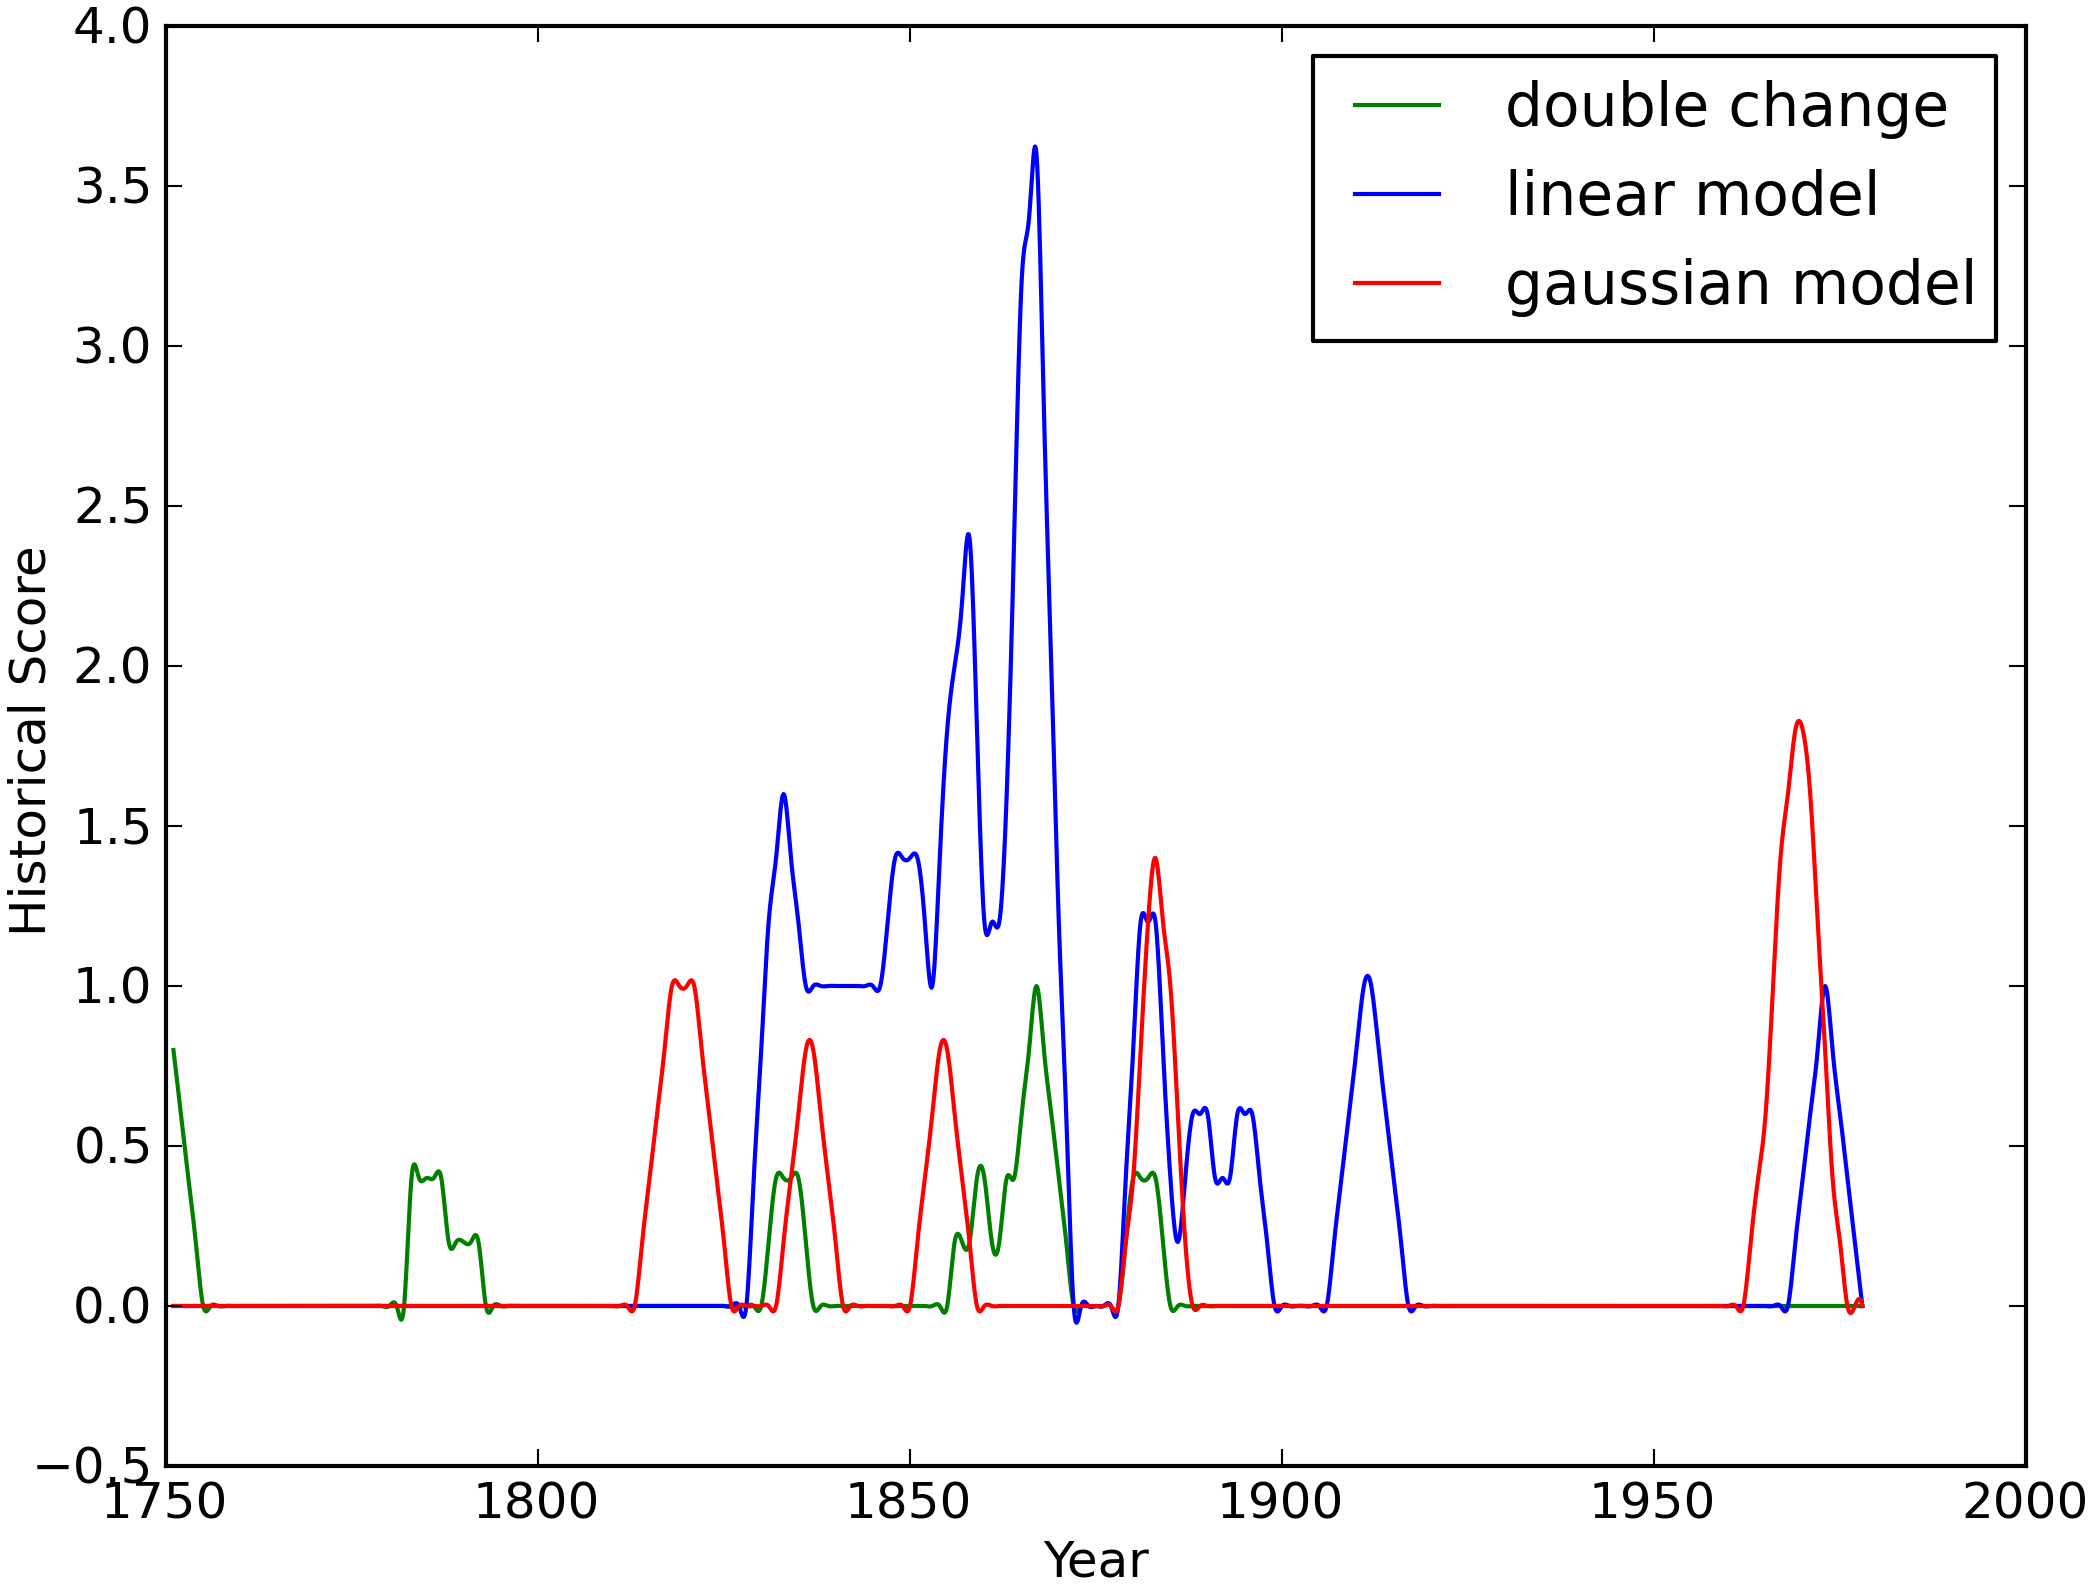
\includegraphics[max size={0.8 \textwidth}{0.8 \textheight}]{slavery-relevance}
\caption{Historical relevance of slavery}
\label{fig:slavery-relevance}
\end{figure}

Of the three algorithms, it cannot be said that one of the them performs the best at detecting and characterizing peaks. However, with the help of an example such as \autoref{fig:slavery-relevance}, one can point the strengths and weaknesses of each of them (for the Gaussian model, I have used the widening parameter $w = 2$). As it could be seen in \autoref{fig:comparative-series}, slavery has had two important "historic peaks": the first, between $1842$ and $1871$, includes the American Civil War, while the second, between $1964$ and $1979$, includes the African-American Civil Rights Movement.

The first peak is detected by all three algorithms. Since it is triangular in shape, the best detection is performed by the linear model algorithm, since it can be approximated pretty well with 2 lines. The other two algorithms also detect activity in this period, but in 2 distinct intervals. Although it seems the results are worse, it can be noted that the second interval detected by the Gaussian model is centered around the American Civil War. The conclusion that can be drawn from this example is that although the linear model is better at detecting triangular peaks, the Gaussian model does a better job at identifying the high point that probably corresponds to a historic event. The double change model is significantly worse than the other two, since it more likely assigns relevance to the tails of the triangle, rather than to the peak.

The second peak is detected only by the last two algorithms. Although both reasonably identify the peak, the Gaussian model performs better by considering a slightly larger interval. This is to be expected, as the peak is roughly bell-shaped.

Lastly, the double change model also detects a minor peak centered around $1790$. In that period, the Constitution of the United States was drafted, and one if its highlights was the Three-Fifths Compromise, which stated that for representation purposes, slaves counted as only three-fifths of a person. Thus, although theoretically inferior to the other two algorithms, the double change model has the capability of detecting less important historic events.


\subsection{Historically Relevant Documents and Topic Models}

Now that several ways of assigning historical relevance to an n-gram have been developed, the problem of identifying historical events can finally be tackled. For each year $t \in \left[ 1500, 2008 \right]$, we build its historically relevant document $d_t$ as follows: we include each $w_i$ (that satisfies $r_{i, t} > 0$) exactly $r_{i, t}$ times.

However, the sheer size of the documents make it intractable to analyze them by hand. Topic models seem most suitable for solving this problem, as they are designed for discovering the hidden thematic structure in document collections \cite{Blei:2012:PTM:2133806.2133826}. The specific algorithm used in this paper is the Latent Dirichlet Allocation (LDA) \cite{Blei:2003:LDA:944919.944937}. In this generative model, each topic is represented as a multinomial distribution over the words. To generate a document of given length, one first selects a topic mixture from a Dirichlet distribution over all topics. Then, for each word, one selects a topic from the previous topic mixture, which is used for sampling the word.

Upon applying Latent Dirichlet Allocation to the historically relevant documents, ideally the topics found by the algorithm should be types of historic events and the topic distribution for any given year should represent the underlying historic events going on in that year. However, what ends up happening is that recurrent themes for consecutive years are grouped into a topic. While this still needs the intervention of a human to interpret the results, the data that must be analyzed is significantly smaller in size. Thus, for every period in time, we will get a set of keywords, some of which will point to historic events, while others may point to cultural trends.
